\section{Struttura precedente}

La struttura sulla quale è stato basato il progetto è locata sul lago di Endine,  precisamente nel comune di Spinone in via Nazionale 56. Nella \cref{fig:streetview} possiamo vedere una fotografia\footnote{Da StreetView: www.maps.google.com} in cui è mostrata la plausibile locazione del progetto.

L'edificio esistente è un edificio privato, dalle dimensioni di $4.30 \times 5.40$ metri, che in precedenza era adibito a rimessaggio per le barche.  È stato scelto sulla base della sua posizione perché dista pochi metri dal lago, è immersa in un ampio spazio verde  ed situata di fronte alla pista pedonale. Si tratta di un passaggio molto frequentato  che permette di percorrere tutto il lago, rendendo cosi il luogo di facile accesso per turisti e passanti. Infatti nei periodi estivi diventa un luogo di svago e relax per famiglie e gruppi. La zona circostante è pubblica e risulta già allestita con tavoli e panchine. Alle spalle vi è un vialetto  che si collega alla strada principale, permettendo così di raggiungere facilmente la struttura e offrendo dei parcheggi.

\begin{figure}[H]
	\centering
	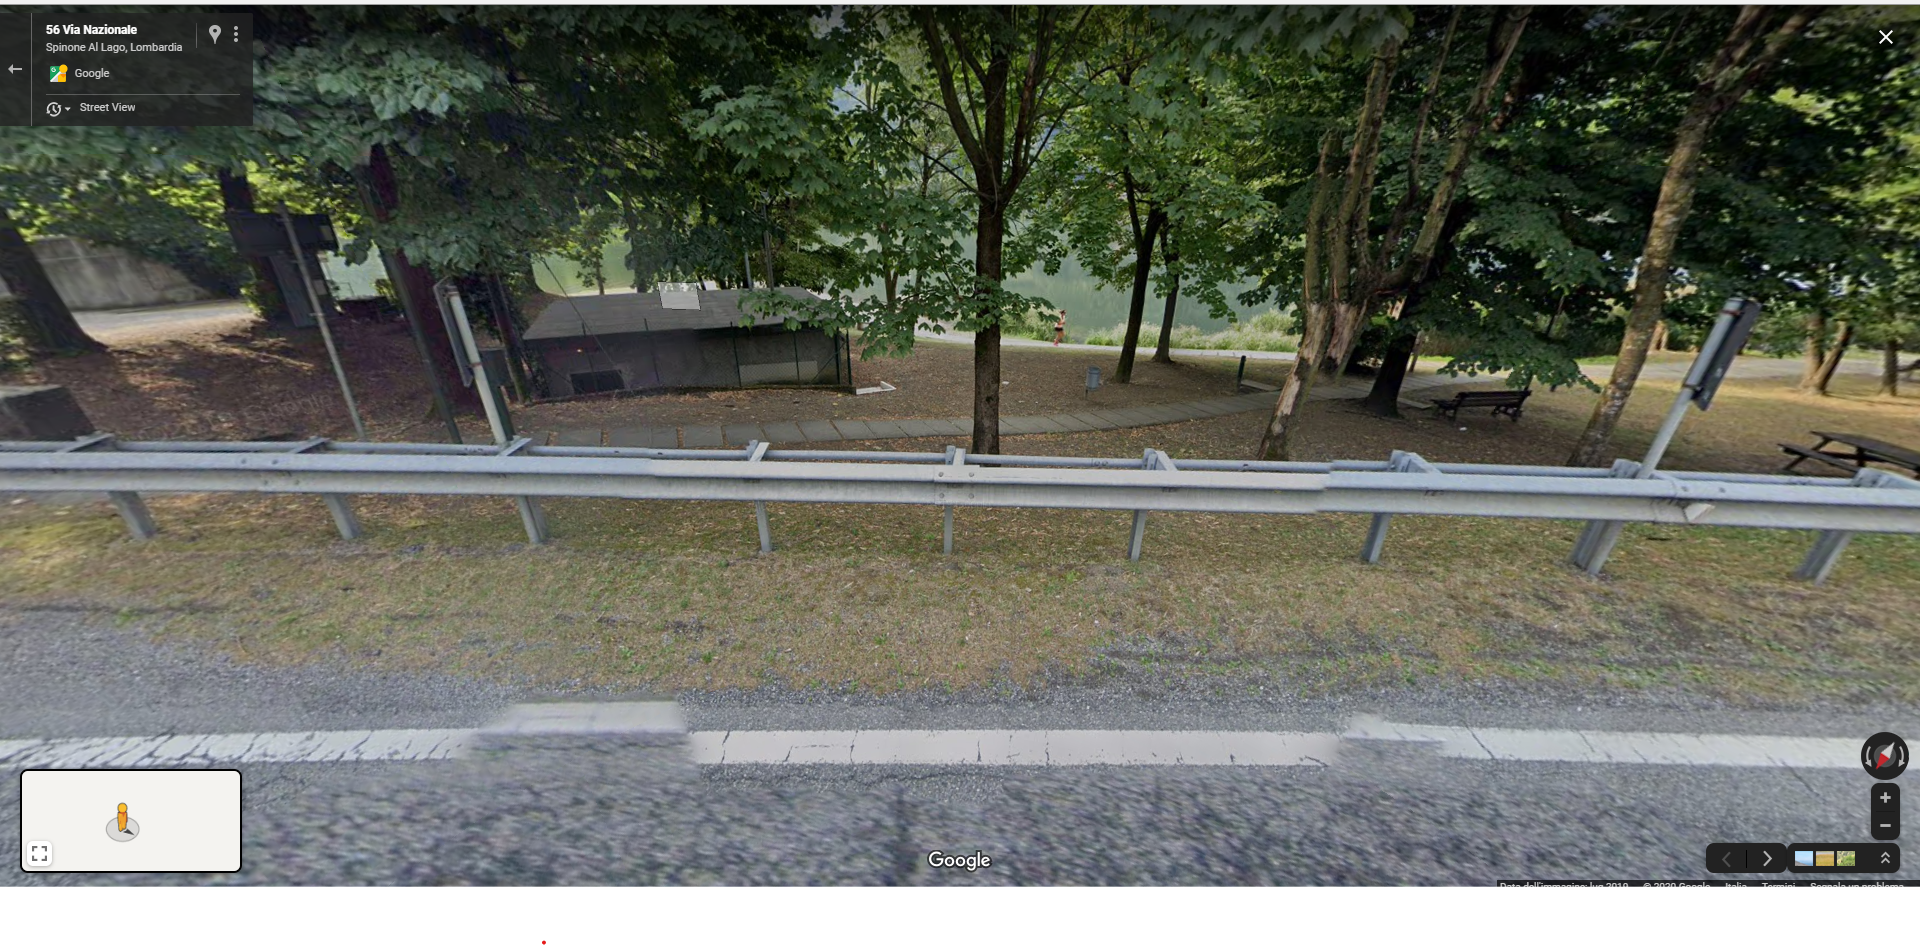
\includegraphics[width=0.8\textwidth]{image11}
	\caption{Street view}
	\label{fig:streetview}
\end{figure}

\clearpage
\subsection{Collocazione}

L'edificio per il rimessaggio (\cref{fig:rimessaggio} [b])si trova sul versante ovest del lago. Gode di un'ottima posizione ed esposizione alla luce solare.

\begin{figure}[H]
	\captionsetup[subfloat]{farskip=2pt,captionskip=8pt}
	\centering
	\subfloat[Lago di Endine]{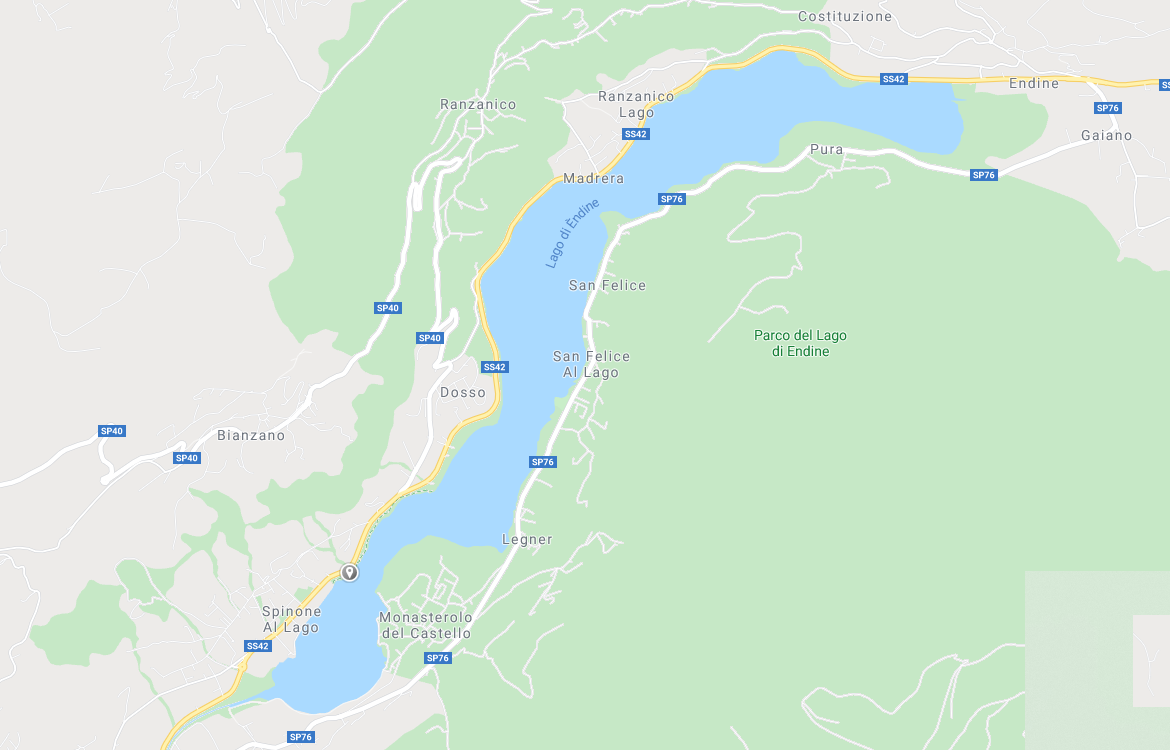
\includegraphics[width=6cm]{image12}}
	\hspace{1cm}
	\subfloat[Edificio preesistente]{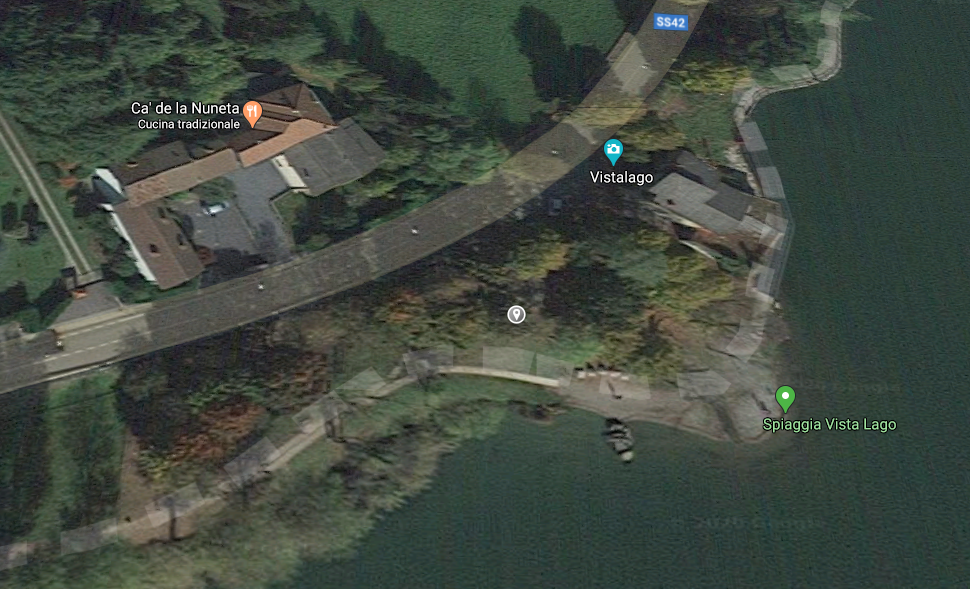
\includegraphics[width=6cm]{image24}}
	
	\caption{Immagini dall'alto}
	\label{fig:rimessaggio}
\end{figure}


\begin{figure}[H]
	\centering
	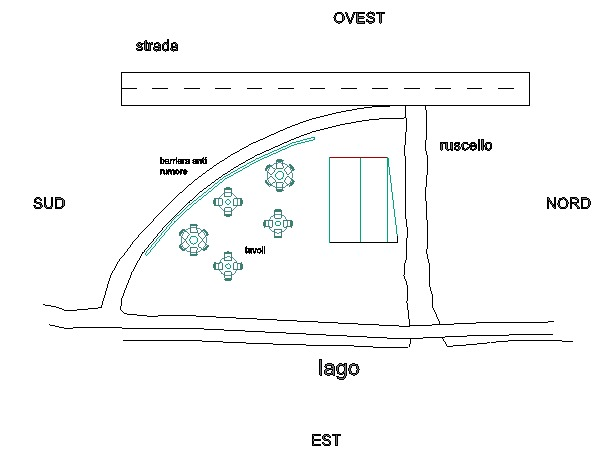
\includegraphics[width=0.8\textwidth]{image100.jpeg}
	\caption{Planimetria} 
	\label{fig:mesh1}
\end{figure}